% ------------------------------------------------------------------------------
% LaTeX template created by
% Iker Algañaraz, May Juarez F., Gastón A. Lozano S., Belén N. Paz
% ------------------------------------------------------------------------------

\documentclass[a4paper,12pt]{article}

% ------------------------------------------------------------------------------
% Packages
% ------------------------------------------------------------------------------
\usepackage{anysize} % Márgenes
\usepackage[hypcap=false, font=small, justification=centering, labelfont=bf]{caption} % Pie de foto/tabla
\usepackage{multicol} % Columnas
\usepackage{amsmath} % Fórmulas matemáticas
\usepackage{amssymb} % Símbolos matemáticos
\usepackage{amsfonts} % Font matemática
\usepackage[utf8]{inputenc} % Facilitar la escritura en español
\usepackage{xcolor} % Color del texto
\usepackage{graphicx} % Figuras
\usepackage[spanish,es-tabla]{babel} % Tipografía del idioma
\usepackage{booktabs} % Separación en tablas
\usepackage{multirow} % Multirow en tablas
\usepackage{hyperref} % Refs como hyperlinks
%\usepackage{biblatex} % Bibliografía automática a partir de base bib

%\usepackage{array}
%\usepackage{verbatim}% Comentarios multilinea
%\usepackage{siunitx} % Unidades del sistema internacional
%\usepackage{fancyhdr} % Personalizar encabezado y pie de pagina
%\usepackage{longtable} % Tablas largas
%\usepackage{blindtext} % Lore ipsum
%\usepackage{soul} % Subrayar
%\usepackage{grffile}
%\usepackage{mathrsfs}

% ------------------------------------------------------------------------------
% Config
% ------------------------------------------------------------------------------
\newenvironment{Figure}
  {\par\medskip\noindent\minipage{\linewidth}}
  {\endminipage\par\medskip}

\providecommand{\abs}[1]{\lvert#1\rvert} % Valor absoluto

\marginsize{2cm}{2cm}{1cm}{2cm} % pkg: anysize

\graphicspath{{./Fotos/}} % pkg: graphicx

\setlength\columnsep{18pt}
\setlength\parskip{4pt} \setlength\parindent{0in}

\title{Tour por el espectro electromagnético\\ 
\medskip \large Universidad Nacional de Tucumán}
\author{May Juarez Ferriol}
\date{}

% ------------------------------------------------------------------------------
% Document
% ------------------------------------------------------------------------------
\begin{document}

\maketitle

\section*{Introducción}

La energía electromagnética se manifiesta como ondas que se desplazan a través del espacio, abarcando un espectro asombrosamente amplio, que se extiende desde las ondas de radio hasta los rayos gamma. Sin embargo, a pesar de la vastedad de este espectro, la vista humana solo es capaz de percibir una pequeña porción conocida como luz visible.

Cada dispositivo que utilizamos, ya sea una radio, una televisión o una máquina de rayos X, se encuentra sintonizado para interactuar con una parte específica de este espectro electromagnético. La agencia espacial NASA utiliza instrumentos científicos que se aprovechan de todo el rango del espectro electromagnético para estudiar la Tierra, nuestro sistema solar y más allá, desvelando los misterios del universo con la ayuda de esta energía.

\medskip

\begin{multicols*}{2}

\section*{Ventanas atmosféricas}

Las ventanas atmosféricas son rangos específicos del espectro electromagnético a través de los cuales la atmósfera terrestre permite que la radiación electromagnética llegue hasta la superficie de la Tierra sin ser absorbida o bloqueada en gran medida. Estas ventanas atmosféricas son importantes porque permiten la observación de objetos celestes y la transmisión de señales de comunicación a través de la atmósfera. 

\begin{Figure}
    \centering
    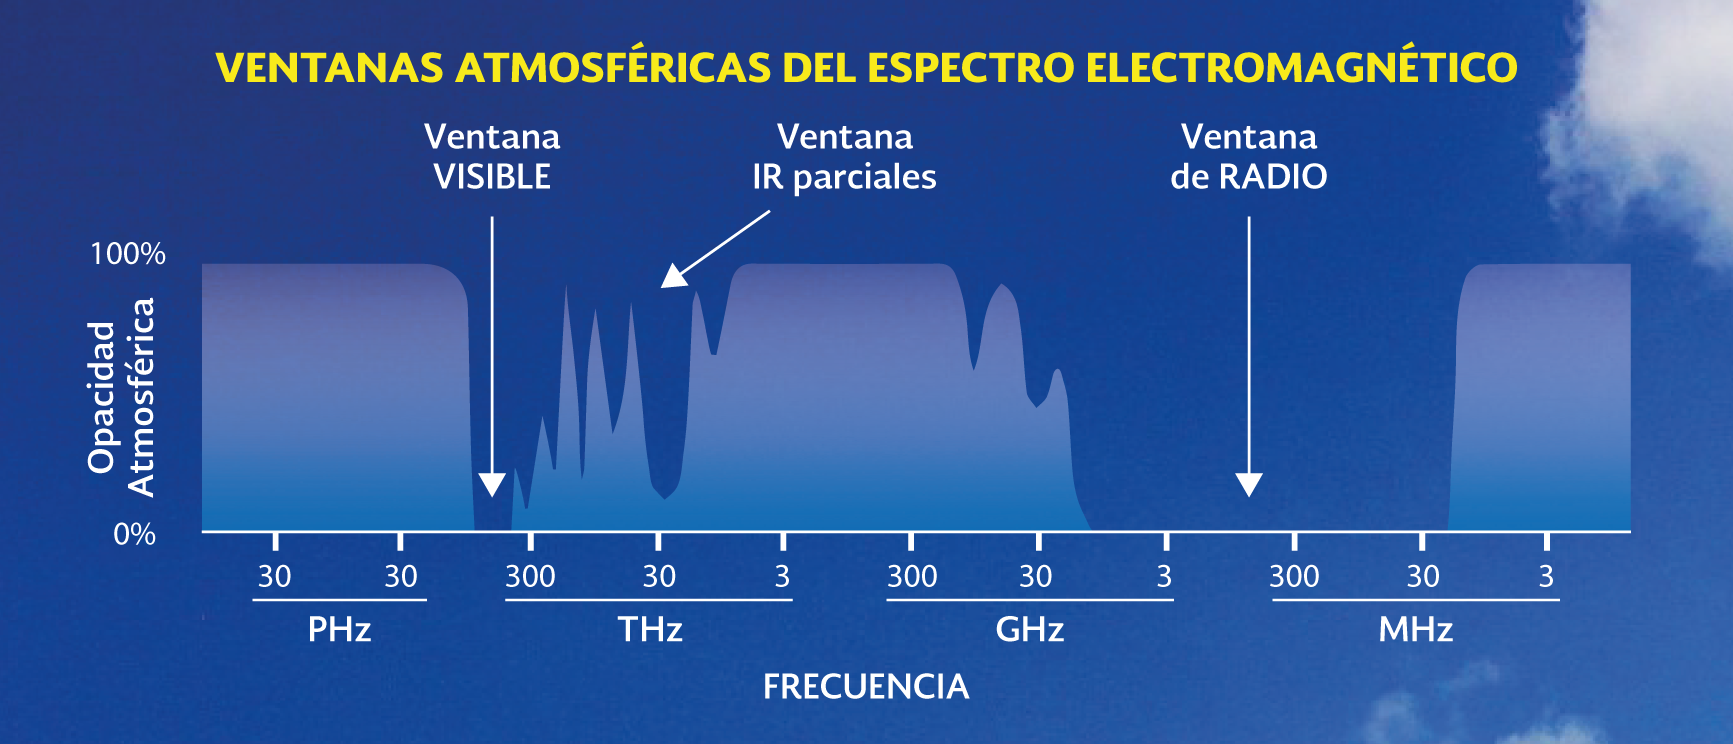
\includegraphics[width=1\linewidth]{VentanasAtmosfericas.png}
    \captionof{figure}{\textit{Ventanas atmosféricas} [Figura], por Muñoz, 2014: Ventanas atmosféricas del espectro electromagnético}
    \label{fig: ventAtmos}
\end{Figure}

Las ventanas atmosféricas se ubican en diferentes partes del espectro electromagnético y tienen diferentes extensiones. Algunas de las ventanas atmosféricas que podemos mencionar son:

La ventana de radio: Esta ventana se extiende en el rango de radio del espectro electromagnético, que abarca desde aproximadamente unos pocos kHz hasta varios GHz. Es esencial para la transmisión de señales de radio y comunicación inalámbrica, y más cerca de la región de las microondas, también puede ser utilizada para la comunicación por satélite y la radiodifusión de televisión por satélite.

La ventana de infrarrojo: Esta ventana se extiende desde el infrarrojo cercano hasta el infrarrojo medio, abarcando longitudes de onda de aproximadamente 10 micrómetros. Es importante para la observación de objetos celestes, la teledetección ambiental y la termografía.

\newpage

La ventana óptica: Esta ventana se encuentra en la región del espectro electromagnético que abarca desde la luz visible hasta el infrarrojo cercano. Incluye las longitudes de onda visibles por el ojo humano y es fundamental para la observación astronómica y la vida cotidiana.

Estas ventanas atmosféricas son cruciales porque permiten que la radiación electromagnética de diversas fuentes cósmicas alcance la Tierra y sean detectadas por instrumentos científicos y sistemas de comunicación. Las longitudes de onda fuera de estas ventanas tienden a ser absorbidas por moléculas y partículas en la atmósfera, lo que hace que sea difícil o imposible observar o transmitir señales a través de ellas.

\subsection*{El espectro visible}

El espectro visible se encuentra dentro de una de las ventanas atmosféricas más importantes y conocidas. El espectro visible abarca longitudes de onda aproximadamente en el rango de 380 a 750 nanómetros. Esta es la región del espectro electromagnético que es perceptible por el ojo humano y contiene los colores del arcoiris: violeta, azul, celeste, verde, amarillo, naranja y rojo.

\begin{Figure}
    \centering
    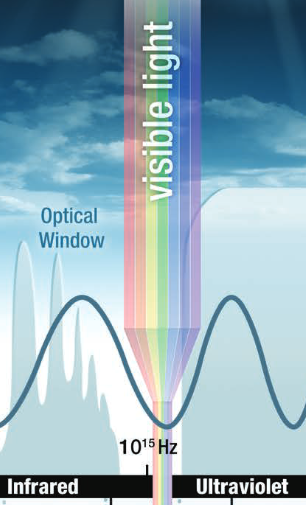
\includegraphics[width=0.5\linewidth]{EspectroVisible.png}
    \captionof{figure}{\textit{Espectro visible} [Figura], por Butcher, 2016: Tour of the electromagnetic spectrum}
    \label{fig: especVisible}
\end{Figure}

En términos de la longitud total del espectro electromagnético, el espectro visible es solo una pequeña porción. El espectro electromagnético abarca una amplia gama de longitudes de onda, desde las ondas de radio con longitudes de onda mucho más largas hasta los rayos gamma con longitudes de onda extremadamente cortas. A pesar de su pequeña extensión en términos de longitudes de onda, el espectro visible es fundamental para la percepción visual y la observación de objetos y fenómenos en el mundo que nos rodea.

\section*{Energía electromagnética}

La energía electromagnética se describe en términos de frecuencia, longitud de onda y energía en distintas regiones del espectro electromagnético. Las tres están relacionadas matemáticamente de manera que si sabes una, podes calcular las otras dos.

\begin{Figure}
    \centering
    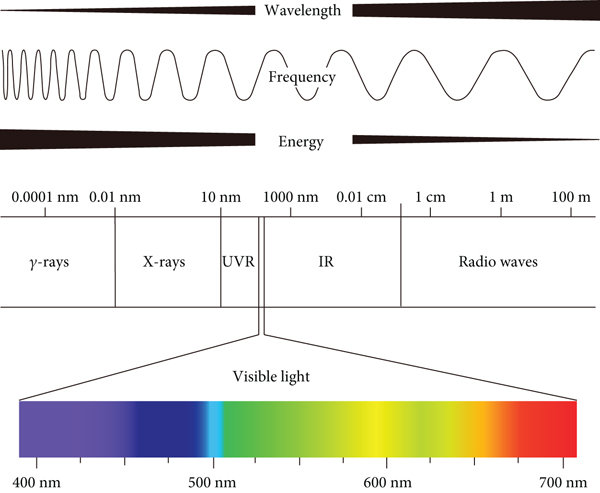
\includegraphics[width=1\linewidth]{WaveFreqEnergy.jpg}
    \captionof{figure}{\textit{Frecuencia, longitud de onda y energía en el espectro electromagnético} [Figura], por Bo Yu, 2022: The relationship between photon energy and wavelength}
    \label{fig: WaveFreqEnergy}
\end{Figure}

La frecuencia se utiliza para describir regiones del espectro electromagnético como las ondas de radio y las microondas. La frecuencia se mide en Hertz (Hz), que representa el número de ciclos completos que pasan por un punto en un segundo. Esta medida es especialmente útil en el caso de las ondas de radio y las microondas porque estas frecuencias son relativamente bajas y varían desde kilohertz (kHz) hasta gigahertz (GHz). %El uso de la frecuencia facilita el cálculo de otras propiedades como la longitud de onda y la energía.

La longitud de onda se aplica a las regiones del espectro electromagnético que incluyen el infrarrojo y la luz visible. Aquí, la longitud de onda se mide en metros y se refiere a la distancia entre dos picos consecutivos de una onda. Esta medida es adecuada para describir la luz visible porque diferentes colores de luz tienen longitudes de onda distintas. Esta relación permite comprender cómo la longitud de onda influye en la percepción visual de los colores.

La energía se emplea para describir regiones del espectro que incluyen los rayos X y los rayos gamma. La energía se mide en electronvoltios (eV) y cuantifica la cantidad de energía transportada por los fotones en estas regiones de alta energía. A medida que avanzamos desde longitudes de onda más largas hacia las más cortas, la energía aumenta significativamente. Esto es esencial en aplicaciones médicas, como la radiología, donde los rayos X de alta energía pueden penetrar tejidos para fines de diagnóstico.

La elección de estas expresiones es una convención científica que facilita la descripción y la comprensión de las propiedades de las ondas electromagnéticas en cada región del espectro. Esto permite a los científicos y tecnólogos utilizar unidades de medida apropiadas para las características específicas de cada tipo de radiación electromagnética, asegurando que los números involucrados en los cálculos no sean ni demasiado grandes ni demasiado pequeños, lo que simplifica la representación y la manipulación de datos en estas diversas regiones del espectro electromagnético.

\subsection*{Visualización de la energía}

Para visualizar imágenes que están fuera del rango del espectro de luz visible, se utiliza una escala de colores (normalmente los mismos rojo, azul y verde que se usa en la creación de imágenes naturales), para visualizar distintas longitudes de onda, como por ejemplo una imágen combinada de tres satélites donde una imagen usa el canal rojo (infrarrojo), una el canal amarillo (luz visible), y una el canal azul (rayos x). Es como ver con una cámara, unos lentes de visión nocturna y visión de rayos x todo a la vez.

\begin{Figure}
    \centering
    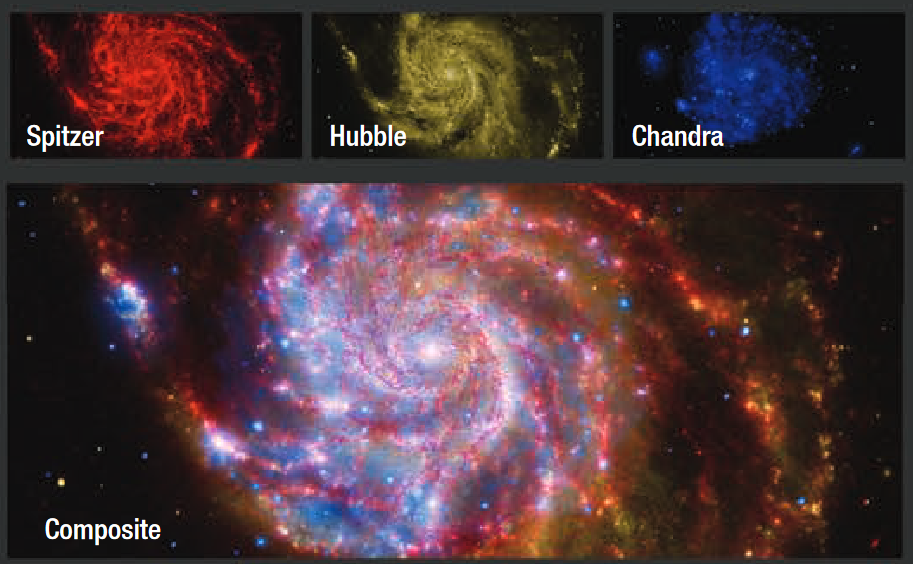
\includegraphics[width=1\linewidth]{satViewComposite.png}
    \captionof{figure}{\textit{Composición de 3 satélites} [Figura], por Butcher, 2016: Tour of the electromagnetic spectrum}
    \label{fig: satViewComposite}
\end{Figure}

\section*{Luz visible}

La determinación de la presencia de elementos de la tabla periódica en el Sol, otras estrellas y planetas se basa en el estudio de los espectros de luz visible que emiten o reflejan. Este estudio se basa en la observación de las líneas de absorción y las características espectrales que se producen en el espectro de luz visible.

Espectros de absorción en el Sol y otras estrellas: Cuando observamos el espectro de luz visible del Sol y otras estrellas, notamos la presencia de líneas oscuras llamadas líneas de absorción. Estas líneas de absorción son causadas por la absorción de ciertas longitudes de onda de luz por elementos presentes en la atmósfera estelar. Cada elemento tiene una firma de líneas de absorción única que actúa como una huella digital que revela su presencia. Los astrónomos comparan estas líneas de absorción con las líneas conocidas de elementos en la Tierra para identificar los elementos presentes en el Sol y otras estrellas.

\begin{Figure}
    \centering
    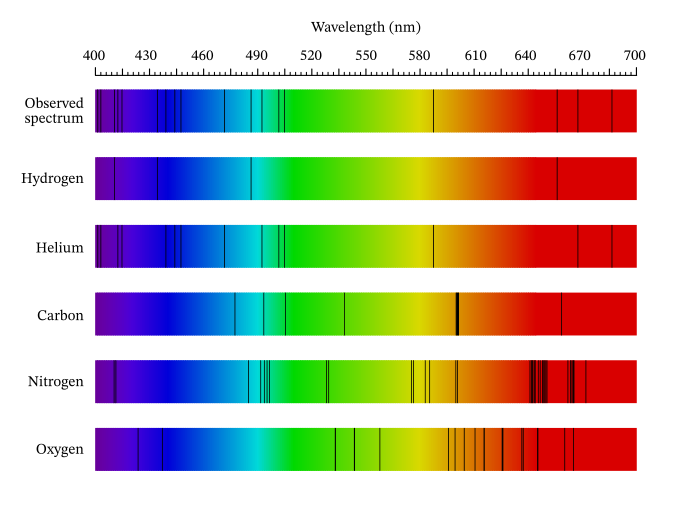
\includegraphics[width=1\linewidth]{AbsorbSpectrum.png}
    \captionof{figure}{\textit{Espectro de absorción para varios elementos comunes} [Figura], por Nagwa, 2023: Emission and absortion spectra}
    \label{fig: AbsorbSpectrum}
\end{Figure}

Espectros de reflectancia en planetas: Cuando se estudian planetas o cuerpos celestes dentro de nuestro sistema solar, se utiliza el espectro de reflectancia. Esto implica observar cómo la luz del Sol se refleja en la superficie del planeta y cómo esa reflectancia varía con diferentes longitudes de onda. Al igual que con las estrellas, los elementos en la superficie de un planeta absorberán y reflejarán luz en patrones característicos que pueden compararse con las firmas espectrales conocidas de elementos y compuestos en la Tierra para determinar su composición.

\begin{Figure}
    \centering
    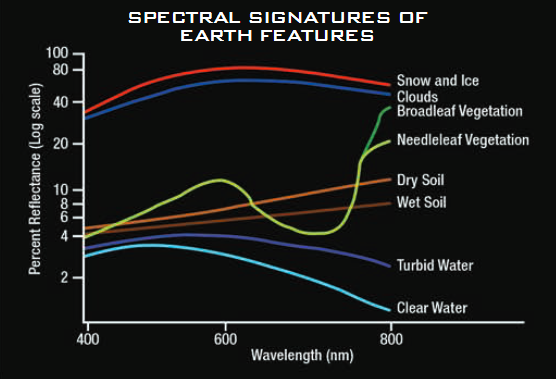
\includegraphics[width=0.9\linewidth]{refSpectrum.png}
    \captionof{figure}{\textit{Espectro de reflectancia de elementos de la Tierra} [Figura], por Butcher, 2016: Tour of the electromagnetic spectrum}
    \label{fig: RefSpectrum}
\end{Figure}

La relación entre el color y la temperatura se basa en la ley de Wien, que establece que la longitud de onda dominante de la luz emitida por un objeto caliente está inversamente relacionada con su temperatura. Esto significa que a medida que un objeto se calienta, su color cambia de manera predecible:

Cuando un objeto se calienta a temperaturas extremadamente altas, emite radiación dominada por longitudes de onda cortas, lo que se traduce en colores azules o incluso ultravioleta. Por ejemplo, el Sol, con una temperatura de aproximadamente 5,500°C, emite luz amarilla.

A temperaturas más bajas, los objetos emiten radiación dominada por longitudes de onda más largas, lo que se traduce en colores más rojos. Por ejemplo, la estrella Betelgeuse es más fría que el Sol y aparece roja.

\begin{Figure}
    \centering
    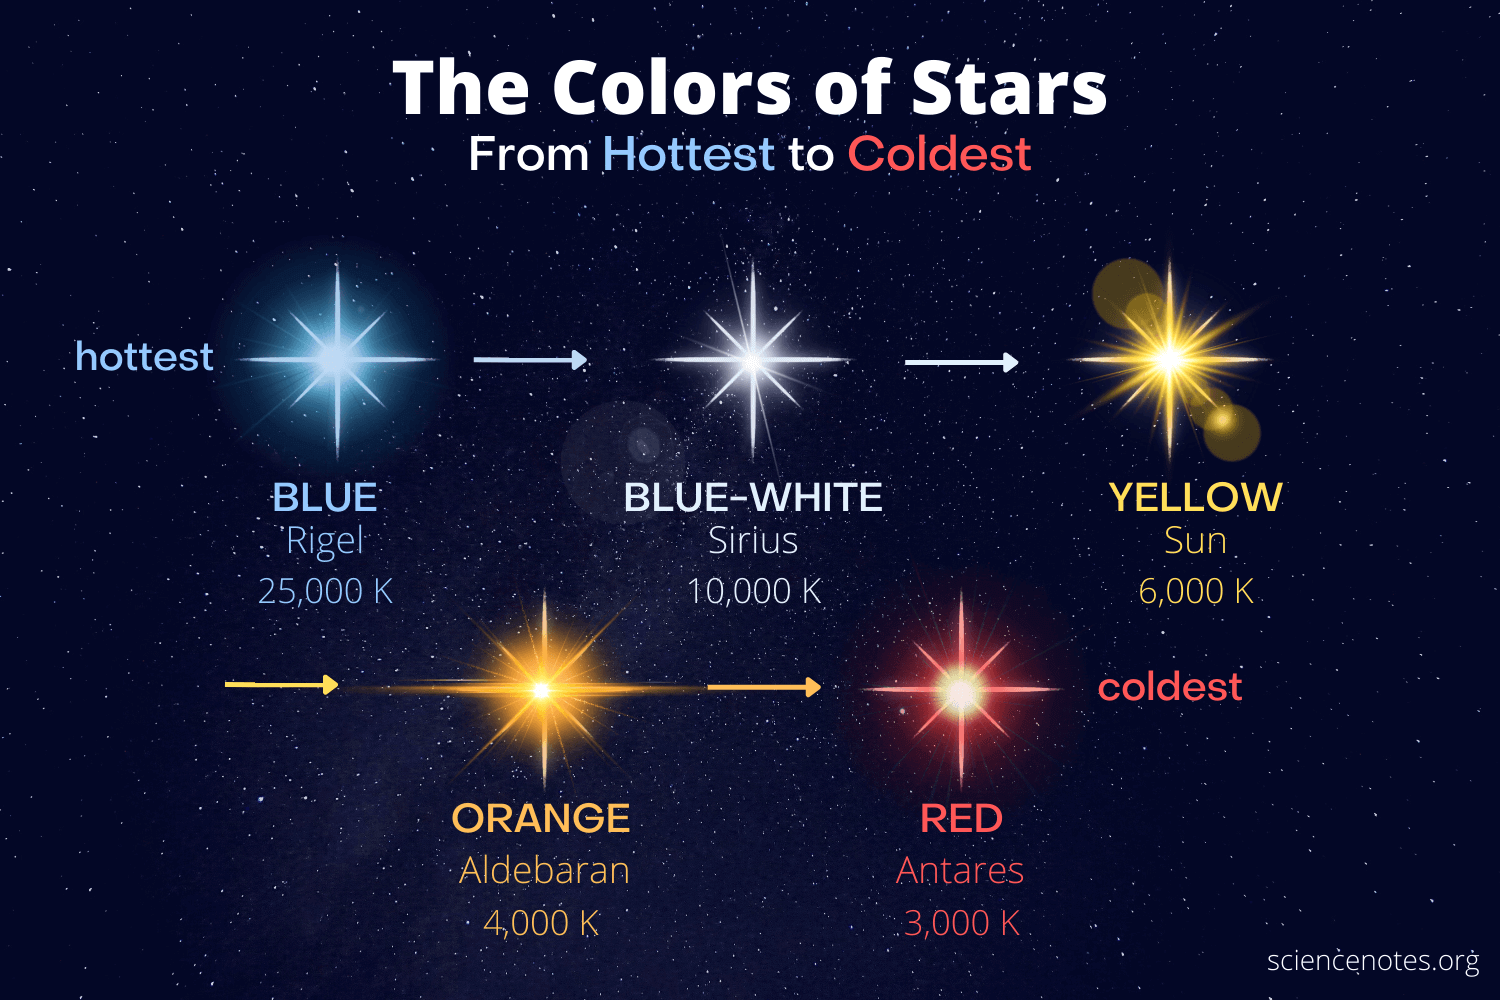
\includegraphics[width=0.9\linewidth]{tempColor.png}
    \captionof{figure}{\textit{Color en base a la temperatura en estrellas} [Figura], por Helmenstine, 2022: The colors of the stars from hottest to coldest}
    \label{fig: tempColor}
\end{Figure}

\begin{thebibliography}{99}

\bibitem{} Butcher. 2016. \emph{Tour of the electromagnetic spectrum}, 1st ed. NASA.

\bibitem{} Muñoz. 2014. \emph{Frecuencias de comunicación satelital}, AEM.

\bibitem{} Bo Yu. 2022. "The relationship between photon energy and wavelength" \emph{Oxidative Medicine and Cellular Longevity}, Hindawi.

\bibitem{} Nagwa. 2023. \emph{Lesson explainer: Emission and Absorption Spectra}. 

\bibitem{} Helmenstine, 2022. \emph{The colors of the stars from hottest to coldest}.

\end{thebibliography}

\end{multicols*}

\end{document}

% ------------------------------------------------------------------------------
% Common references and examples
% ------------------------------------------------------------------------------
% 
% ---------------------------
% Bibliography
% ---------------------------
% \bibitem{} Sears, Zemansky. \emph{Física universitaria}, vol. 2, 14th ed. Pearson Education, 2018.
% \bibitem{} Hecht, Zajac. \emph{Óptica}, 4th ed. Pearson Education, 2003.
% \bibitem{} Serway, Jewett. \emph{Physics for Scientists and Engineers}, vol. 2, 6th ed. Brooks Cole, 2004.
% \bibitem{} Jenkins, White. \emph{Fundamentos de óptica}, 3th ed. Aguilar S.A., 1964.
%
% ---------------------------
% Tables
% ---------------------------
% \begin{Figure}
%     \centering
%
%     \begin{tabular}{c|c}
%         \toprule
%          & \textit{...} \\
%          & \textit{[]} \\
%         \midrule
%         ... & \multirow{2}{*}{$(... \pm ...)$} \\
%         ... & \\
%         ... & \multirow{2}{*}{$(... \pm ...)$} \\
%         ... & \\ \hline
%         ... & $(... \pm ...)$ \\
%         ... & $(... \pm ...)$ \\
%         \bottomrule
%     \end{tabular}
%
%     \captionof{table}{}
%     \label{tab:}
% \end{Figure}
%
% \begin{Figure}
%     \centering
%
%     \begin{tabular}{cc}
%         \toprule
%         \textit{\textbf{... []}} & \textit{\textbf{$... []}}\\
%         \midrule
%         $... \pm ...$ & $... \pm ...$ \\
%         $... \pm ...$ & $... \pm ...$ \\
%         \bottomrule
%     \end{tabular}
%
%     \captionof{table}{}
%     \label{tab:}
% \end{Figure}
%
% ---------------------------
% Figures
% ---------------------------
% \begin{Figure}
%     \centering
%     \includegraphics[width=1\linewidth]{.jpg}
%     \captionof{figure}{}
%     \label{fig:}
% \end{Figure}
%
% ---------------------------
% Equations
% ---------------------------
% \begin{equation}
%     \label{eq:}
%     ...
% \end{equation}
%